\section{Dataset and Methodologies}~\label{sec:approach}

In this section, we present how our dataset is constructed and how the information regarding a-groups and m-groups is collected for comparison.

\subsection{Dataset: a-groups and m-groups}
Our study subject is {\it crash dumps}.  When a crash occurs at the client side, a crash dump is generated by the deployed crash management system. Typically, it captures the program state at the crash as well as static information about the system and software. For example, a crash dump returned by Mozilla Crash Reporter mainly include: 1) call stacks of each active thread at the crash, 2) exception types captured at the crash such as EXCEPTION\_ACCESS\_VIOLATION\_WRITE, and 3) operating system, software and their versions, as well as the building, installation and crashing dates and time.  When a user clicks the {\it submit crash report} button, the crash dumps are sent back to the server for postmortem analysis.  Mozilla Crash Reporter system organizes groups of crash dumps based on applications. For each application, it ranks most frequently occurred crash dump groups within a certain time window. 

A user can also send in crash information manually through Bugzilla~\cite{bugzilla}, in which case, the crash information is constructed in ad-hoc based on the users' judgment. Compared to crash dumps generated automatically, the report in Bugzilla may contain additional information, such as 1) reproduce steps that lead to crashes, 2) piece of code that is suspected to cause the crash, 3) the URL visited when the application crashes, 4) expected results, 5) the other bugs that may be relevant, and 6) any connections to groups of crash dumps reported by Mozilla Crash Reporter. 

In Figure~\ref{fig:dataprocess}, we show how a-groups and m-groups in our study are constructed. The groups of crash dumps are selected from both Mozilla Crash Reporter and Bugzilla, dated between 2/16-4/16/2012, across five applications including {\it Firefox}, {\it Thunderbird}, {\it Fennec}, {\it FennecAndroid} and {\it SeaMonkey}. For a-groups, we collect maximally 300 top crash dump groups for each application. 


For m-groups, we inspect the summary page Mozilla presents for each a-group, shown in Figure~\ref{fig:bugzilla}. From the page, we find Bugzilla entries that are correlated to the a-group, shown in Figure~\ref{fig:bugzilla}. We recursively search each correlated Bugzilla entry to find more Bugzilla entries that are confirmed to be relevant. The crash dumps reported in these Bugzilla entries constitute an m-group. As an example, in Figure~\ref{fig:dataprocess}, $b_1$ and $b_2$ are the two Bugzilla entries found relevant to {\it a-group} and $b_3$ is identified by recursively inspecting $b_1$ and $b_2$ for related bugs. The Bugzilla entries also contain the developers' discussions on how to diagnose the crash dumps. 

\begin{figure}[!htb]
\centering
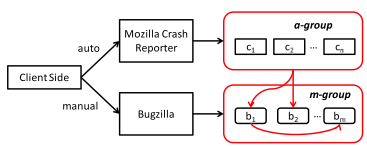
\includegraphics[width = 8.4cm, angle = 0]{approach1.ps}
\caption{\small Collect a-Groups and m-Groups~\label{fig:dataprocess}}
\normalsize
\end{figure}

\begin{figure}[!htb]
\centering
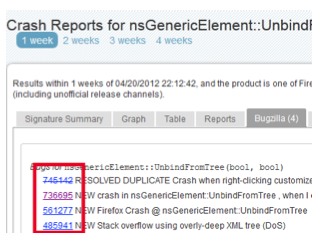
\includegraphics[width = 5.4cm, angle = 0]{bugzilla.ps}
\caption{Link a-group and m-group~\label{fig:bugzilla}}
\normalsize
\end{figure}

Table~\ref{tab:dataset} summarizes the dataset we collected. Under {\it T$_g$}, we display the number of a-groups and m-groups studied for each application. The first four applications contain more than 300 a-groups and by setting a threshold 300, we successfully collected 297 to 299 a-groups. For each application, we randomly select 20 a-groups, based on which we construct m-groups, as explained in Figure~\ref{fig:dataprocess}. Under {\it T$_b$}, we count the total number of Bugzilla entries associated with the 20 m-groups. In each Bugzilla entry, users can report multiple crash dumps related to the bug. Under {\it T$_c$}, we list the total number of crash dumps in the m-groups. The data indicate that on average, each Bugzilla entries contain 2--3 crash dumps.

\begin{table}
\caption{Dataset from 5 Mozilla Applications\label{tab:dataset}}
\resizebox{\columnwidth}{!}{
\begin{tabular}{|l||c|c||c|c|c|}\hline

\multirow{2}{*}{Program} & \multicolumn{2}{|c||}{a-Groups} & \multicolumn{3}{|c|}{m-Groups} \\\cline{2-6}

&T$_g$&T$_c$&T$_g$&T$_b$&T$_c$ \\ \hline\hline

Firefox 14.0a1&298&18316&20&110&233\\ \hline
Thunderbird 10.0&299&3151&20&106&237\\ \hline
Fennec 2.1.2&299&2567&20&87&155\\ \hline
Fennec Android 13.0a1&297&4925&20&90&189\\ \hline
SeaMonkey 2.7.2&257&514&20&59&144\\ \hline

%Firefox 14.0a1&299&18316&1&16/8645&1743&12&20&110&233&3&39&&61\\ \hline
%Thunderbird 10.0&299&3151&16&16/355&1792&32&20&106&237&3&33&1024&93\\ \hline
%Fennec 2.1.2&299&2567&1&16/2233&1792&2&20&87&155&3&24&1456&46\\ \hline
%Fennec Android 13.0a1&168&4925&1&16/993&1165&2&20&90&189&3&24&1456&82\\ \hline
%SeaMonkey 2.7.2&257&514&1&15/15&196&5&20&59&144&3&16&596&6\\ \hline

\end{tabular}
}
\end{table}

\subsection{Comparison Metrics and Approaches}
Given dataset a-groups and m-groups, our goals are to determine whether manual and automatic approaches apply consistent criteria and information to group crashes, and whether the two approaches correlate same types of call stacks. As shown in Figure~\ref{fig:approach}, we compare the groups based on the four metrics, including: 
\begin{itemize}
\item {\it Grouping criteria}: why do we group crash dumps and how the groups can be used?
\item {\it Grouping information}: what information shall we use, and how shall we use it, for more effectively grouping crash dumps?
\item {\it Imprecision in the groups}: when do we group unrelated crash dumps or when do we fail to find the relevant crash dumps? 
\item {\it Characteristics of call stacks}: what are the patterns in call stacks in a-groups and m-groups? How do the characteristics imply the capabilities of the two approaches?
\end{itemize}


\begin{figure}[!htb]
\centering
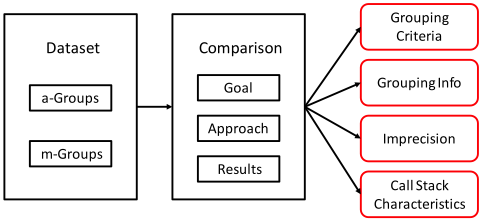
\includegraphics[width = 8.4cm, angle = 0]{approach2.ps}
\caption{Compare a-Groups and m-Groups~\label{fig:approach}}
\normalsize
\end{figure}

To collect information for performing comparisons, we take the following three steps.

{\bf Identifying grouping criteria and information.} For a-groups, we studied documentation related to Mozilla Crash Reporter to understand the criteria and algorithms used. To determine grouping criteria and information used for m-groups, we analyzed  452 Bugzilla entries where the m-groups are determined. For learning grouping criteria, our focus is to determine what relations are established between crash dumps in the group and how developers compare and contrast crash dumps in a group for prioritizing, diagnosing and fixing the code. To obtain information important for correlating crash dumps, we define a set of keywords, representing potential sources of information,  e.g., {\it call stacks}, {\it reproduce steps}, {\it regression windows}, {\it URL}, {\it plugin} and {\it libraries}. Based on these key words, we extract relevant text from the Bugzilla entries. We then count the frequencies at which each type of information is used and also the frequencies at which different types of information are combined in determining a group.

{\bf Determining imprecision in a-groups and m-groups.} In this step, we aim to learn the existence, causes and consequences of imprecision for both of the approaches. To determine imprecision in a-groups, we randomly selected 100 a-groups from our dataset and for each a-group, we analyze the relevant Bugzilla entries that contain diagnostic information for the a-groups. We determine an a-group is imprecise if the developers confirm that the a-group: 1) contains a corrupted signature or call stack, 2) includes crash dumps that should not be correlated, and 3) fails to group crash dumps that should be correlated.  Imprecision in m-groups is caused by developers' mistakes. We inspect developers' discussion logs in the Bugzilla entries and identify cases where developers believe unrelated crash dumps are grouped by mistakes.

{\bf Comparing call stack characteristics.} To compare the capabilities of manual and automatic approaches, we study the patterns in call stacks for a-groups and m-groups. To determine if there is a pattern, we also construct {\it r-groups}; each of the r-groups contains the random number of crash dumps randomly selected from a-groups.  We compare a-groups and m-groups regarding 1) the sizes of groups, including the number of call stacks in each group and the length of the call stacks, and 2) the similarity between call stacks. We compute the metrics in string matching algorithms to measure the similarity between the call stacks, including the {\it Brodie value} ({\it B-Value}), {\it Brodie weight} ({\it B-Weight})~\cite{brodie:automated,brodie:quickly}, longest common substrings ({\it LCS}), and the percentage of identical call stacks in a group ({\it C-Identical}). In the following, we explain how each of the measure is calculated. 

Suppose $m$ is the number of {\it matching lines} between two call stacks, and $l_1$ and $l_2$ are the lengths of the two call stacks. Brodie value $bv$ is computed as:

\[
  bv = \left\{
  \begin{array}{l l}
    m/l_1 & \quad l_1 == l_2\\
    m/((l_1+l_2)/2) & \quad l_1\neq l_2\\
  \end{array} \right.
\]

We consider a {\it matching line} between two call stacks if at location $i$ from the top of the call stacks $C_1$ and $C_2$, the function names $C_1[i]$ and $C_2[i]$ are identical. 

Brodie weight is a string similarity metric improved from the Brodie value. It distinguishes the weight of the functions in call stacks for determining similarity. The assumption is that functions located at the top of the call stack should have more weight than ones located at the bottom. The detailed algorithm of how to compute Brodie weight between two call stacks is given in~\cite{brodie:automated}.

%\IncMargin{1em}
%\LinesNumbered
%\begin{algorithm}[!htb]
%\SetFuncSty{bf}
%\SetKwData{ans}{Unsolved}
%\SetKwFunction{icfg}{BuildICFG}
%\SetKwInOut{Input}{Input}
%\SetKwInOut{Output}{Output}

%\Input{Specification of Fault, $spec$}
%\Output{Calls to {\bf MatchFSignature}, {\bf MatchDSignature};\\

%A repository of function definitions, $R$}
%\BlankLine
 	  
%\caption{Generating Analysis\label{alg:generation}} %{\bf MatchFSignature} and {\bf MatchDSignature}
%\normalsize
%\end{algorithm}

We obtain the Brodie value/weight for a group by adding up the Brodie value/weight for every two call stacks in the group and then dividing the times of comparisons. Finally, we get an average across groups for an application.

To compute LCS across all the call stacks in a group, we first detect a set of common substrings between two call stacks. We then determine whether other call stacks in the group contain the same common substrings. The comparison is performed between the average LCS across a-groups and the average LCS across m-groups for an application. 

The {\it C-Identical} identifies the maximum number of crash dumps in a group that are actually identical, calculated by $n_i$/$n$. In an a-group or m-group, we may find several subgroups, within which, crash dumps are identical. $n_i$ here is the number of identical call stacks in the largest subgroup and $n$ is the size of the a-group or m-group.